%Бумага A4, шрифт 14
\documentclass[a4paper,15pt]{article}
\usepackage{cmap}
\usepackage{mathtext}
%\usepackage{cyrtimes}
\usepackage{listings}
\usepackage{xcolor}
\usepackage{textcomp}
\usepackage[T2A]{fontenc}
\usepackage[utf8]{inputenc}
\usepackage{setspace}
\usepackage[english,ukrainian]{babel}
\usepackage{amssymb,amsfonts,amsmath,cite,enumerate,float,indentfirst, mathtools}
\usepackage{icomma} 
\usepackage{graphicx}
\usepackage{caption}
\usepackage[compact,explicit]{titlesec}
\usepackage{euscript}
\usepackage{mathrsfs}
\usepackage{fancybox}
\usepackage{hyperref}
\mathtoolsset{showonlyrefs=true}
%Оформление библиографии через точку
\makeatletter
\renewcommand{\@biblabel}[1]{#1.}
\makeatother

%Полуторный интервал
\renewcommand{\baselinestretch}{1.4}

%Растягивать там, где не удается перенести слово
\sloppy

%Частота переносов
\hyphenpenalty=2000

\parindent 1cm  %абзацный отступ

%Отступы у страниц
\usepackage{geometry}
\geometry{left=2.5cm}% левое поле
\geometry{right=1cm}% правое поле
\geometry{top=1cm}% верхнее поле
\geometry{bottom=2.5cm}% нижнее поле


\usepackage{fancyhdr}
\pagestyle{fancy}
\fancyhf{}
\fancyhead[C]{}
\setlength{\headheight}{17pt}
\fancyfoot[R]{\thepage}
\renewcommand{\headrulewidth}{0pt}
\renewcommand{\footrulewidth}{0pt}

%Меняем везде перечисления на цифра.цифра
\renewcommand{\theenumi}{\arabic{enumi}.}
\renewcommand{\labelenumi}{\arabic{enumi}.}
\renewcommand{\theenumii}{.\arabic{enumii}.}
\renewcommand{\labelenumii}{\arabic{enumi}.\arabic{enumii}.}
\renewcommand{\theenumiii}{.\arabic{enumiii}}
\renewcommand{\labelenumiii}{\arabic{enumi}.\arabic{enumii}.\arabic{enumiii}.}


\graphicspath{{./img075/},{./img05/}, {./}}
%Пользовательские функции
\newcommand{\addimg}[3]{
\begin{figure}
\begin{center}
\includegraphics[scale=#2]{#1}
\end{center}
\caption{#3}
\end{figure}
}
\newcommand{\addimghere}[3]{
\begin{figure}[H]
\begin{center}
\includegraphics[scale=#2]{#1}
\end{center}
\caption{#3}
\end{figure}
}

\newcommand{\addtwoimghere}[3]
{
\begin{figure}[h]{
\begin{minipage}[h]{0.49\linewidth}
{\includegraphics[width=#3\textwidth]{#1}}
\end{minipage}
%\hfill
\begin{minipage}[h]{0.49\linewidth}
{\includegraphics[width=#3\textwidth]{#2}}
\end{minipage}
	}
\end{figure}
}
\newcommand{\addtwoapp}[3]{
\begin{figure}[h]
\hspace{-15ex}
\begin{minipage}[h]{0.49\linewidth}
{\includegraphics[width=#3\textwidth]{#1}}
\end{minipage}
\hspace{6ex}
\begin{minipage}[h]{0.49\linewidth}
{\includegraphics[width=#3\textwidth]{#2}}
\end{minipage}
\end{figure}

%\begin{figure}[H]
%\begin{center}
%\includegraphics[width=#3]{#1}
%\ %vfill
%\includegraphics[width=#3]{#2}
%\end{center}
%\caption{#4}
%\end{figure}
}

% Cпецифические для курсовой
\newcommand{\upl}[2]{u^{n+1}_{j\ifnum#1=0 ,\else\ifnum#1=1 +1,\else\ifnum#1=-1 -1,\fi\fi\fi k\ifnum#2=1+1\ifnum#2=-1 -1\fi\fi}}
\newcommand{\un}[2]{u^{n}_{j\ifnum#1=0 ,\else\ifnum#1=1 +1,\else\ifnum#1=-1 -1,\fi\fi\fi k\ifnum#2=1+1\ifnum#2=-1 -1\fi\fi}}

%Для кода
\input{listing-python.prf}
\lstset{
language=Python,
belowcaptionskip=\baselineskip,
backgroundcolor=\color{white},
style=python-idle-code,
breaklines=true,
breakatwhitespace=true,
tabsize=2,
numbers=left,
numberstyle=\tiny,
stepnumber=2,
numbersep=8pt,
showstringspaces=false,
frame=tl,
showtabs=false,
framerule=1pt,
rulecolor=\color{black},
captionpos=t,
%keepspaces
}

%В документ включаются различные части работы
\begin{document}
\newpage
\large

\titleformat{\section}[block]{\Large\bfseries\filcenter}{}{1em}{#1}
%\titleformat{\title}[block]{\filcenter\Large\bfseries}{\thesection}{1ex}{\MakeUppercase}

\begin{titlepage}
\paragraph*{}
{\vspace{46pt}}
\begin{center}
\bfseries
{\scshape\Large Національний технічний університет України \\
``Київський політехнічний інститут''\par}
\vspace{12pt}
{\large Фізико-технічний інститут\\}
\vspace{48pt}
{\scshape\Large Курсова\\ \par}
з кредитного модуля <<Методи обчислень>>\\
на тему:\\
{\scshape\Large ``Числове розв’язання диференційних\\
рівнянь у часткових похідних''\\ \par}
Варіант № 8 \\
\end{center}

\vspace{165pt}
\begin{flushright}
\begin{tabular}{rl}
Виконав:\\
студент 3 курсу ФТІ\\
Юрців Ілля Васильович\\
\end{tabular}
\end{flushright}
\vfill
\begin{center}
\bfseries
Київ - 2016
\end{center}
\end{titlepage}

\newpage
\tableofcontents
\newpage

\titleformat{\section}[block]{\Large\bfseries\filcenter}{}{1em}{\thesection\quad#1}
\titleformat{\subsection}[block]{\large\bfseries\filcenter}{}{1em}{\thesubsection\quad#1}
\titleformat{\subsubsection}[block]{\large\bfseries\filcenter}{}{1em}{\thesubsubsection\quad#1}
\titleformat{\paragraph}[block]{\Large\bfseries\filcenter}{}{1em}{#1}

\newcommand{\anonsection}[1]{
\paragraph{#1}\addcontentsline{toc}{section}{#1}
}

\section{Попередній огляд}
\subsection{Постановка задачі}

У даній роботі запропоновано числовий розв’язок р-ня \eqref{eq:fisher}, що моделює процес розмноження бактерій, який
здійснюється шляхом їх ділення.
\begin{equation}
\frac{\partial u}{\partial t} = \alpha (m_{0} -\beta u)u + \sigma\Delta u; \label{eq:fisher}
\end{equation}
Надалі будемо вважати, що процес відбувається в прямокутній  області $\Omega \in \mathbb{R}^{2} $  $(0 \le x \le a, \\
0 \le y \le b)$. Змінна $u$ позначає концентрацію мікроорганізмів у визначеній області.
Порогове значення концентрації $u_{max}=\frac{m_{0}}{\beta}$.

Початкові та граничні умови:
\begin{equation}
	\begin{cases} u\rvert_{t=0} = U(\vec{x}),\ &\forall \vec {x} \in \Omega \\
	u\rvert_\Gamma = u_{\Gamma},\ &\Gamma = \partial \Omega \end{cases} 
\end{equation}
де $U(\vec{x})$  --- гладка класу $\mathbf{C}^2(\Omega)$ функція; крім того для узгодженості початкових та граничних умов покладемо $U(\vec{x})\rvert_\Gamma = u_\Gamma$ i вважатимемо, що протягом усьго розвитку системи значення $u_\Gamma$ залишається постійним. \\
%makebox[5pt]{}
%\shadowbox{Примітка:} Конкретні експерименти проводилися з функцією , в якості якої було обрано двовимірну гаусіану.
\subsection{Розгляд рівняння}
Рівняння \eqref{eq:fisher} є узагальненням для двовимірного простору відомого р-ня Фішера (або частковим випадком з квадратичною нелінійністю р-ня Колмогорова-Петровського-Піскунова). В контексті популяційної динаміки одновимірний безрозмірний варіант цього р-ня був розглянутий  Р. Фішером у 1937 р. у \cite{fisher} де \eqref{eq:fisher} було запропоновано для опису просторового росподілу домінантних алелей і був проведений аналіз його розв’язку у вигляді біжучих хвиль. Стислий але змістовний огляд узагальнення цього р-ня Колмогоровим, а також умови існування його розв’язку у вигляді біжучих хвиль для одновимірного випадку можна знайти в \cite{treft}.

Модель, що задається р-ням \eqref{eq:fisher}, відноситься до типу реакційно-діфузійних моделей. Такі моделі поєднують в собі опис просторово розподіленої хімічної (біологічної, тощо) реакції --- в нашому р-ні представлена логістичним нелінійним членом, --- з описом дифузії реагентів через субстрат --- член з лапласіаном у \eqref{eq:fisher}. Зазвичай такі моделі представляються системою ДРЧП, невідомі ф-ї в якій описують концентрації (зазвичай, або ж деяку іншу характеристику) реагентів (видів, популяцій у застосуванні до біології), що взаємодіють між собою і розповсюджуються у просторі. У нашому випадку розглядається одновидова модель розмноження бактерій на площині з одночасною дифузією. Ділення бактерій описується логістичним членом (який є узагальненням звичайної експоненційної моделі), що введений у \eqref{eq:fisher} для врахування граничної спроможності середовища вміщати у себе популяцію. Без цього нелінійного члена \eqref{eq:fisher} являє собою звичайне параболічне р-ня дифузії, тож модель, як було вказано, поєднує в собі опис розмноження бактерій разом з їх одночасним перерозподілом у просторі.

У таблиці нижче наведена інтерпретація параметрів р-ня з точки зору побудови моделі та біологічного змісту останніх, подробиці можуть бути знайдені у \cite{bio}.
\vspace{10pt}
\begin{center}
	\begin{tabular}{|l|l|}
	\hline
	Parameter & Meaning \\
	\hline
	$\alpha$  & Coef. of linear dependency between $\mathbf{R}(u)$ and "nutrient" \\ \hline
	$\beta$ & Coef. between decrease of "nutrient" and increase of population \\ \hline
	$m_{0}$  & Constant of availability of "nutrient" \\ \hline
	$\sigma$ & Coef. of diffusion \\ \hline
	$n_0 = \frac{m_0}{\beta}$ & Limit carrying capacity \\ \hline
	\end{tabular}
\end{center}
\vspace{10pt}
Тут символом $\mathbf{R}(u)$ позначено логістичний член $\alpha m_0u - \alpha\beta u^2$, який називають "growth rate", або темп росту; він визначає характер "реакційного" вкладу у реакційно-дифузних моделях. Як вказано в \cite{bio} для подібних моделей, що розглядаються у біології, саме квадратичні нелінійні члени є найбільш характерними. Зауважимо, що знову згідно \cite{bio} коефіцієнт $ - \alpha\beta$ визначає (оскільки маємо одну популяцію) внутрішньовидову конкуренцію при $\alpha\times\beta > 0$. Для біологів саме цей випадок є найцікавішим для досліджень у даній моеделі. Якщо коеф-т при квадратичному члені є додатнім, то цей випадок описує свого роду ``коменсалізм'', коли взаємодія окремих особин дає позитивний ефект для розвитку обох. Тим не менш цей окремий випадок нами не розглядався детально, оскільки, як показав експеримент, запропонована у роботі схема дискретизації виявляється суттево нестійкою при $\alpha\times\beta < 0$ (зокрема при $\alpha < 0$, навіть для дуже малих значеннях останнього).
\newpage
\section{Вибір скінченнорізницевої схеми. Дискретизація}
\subsection{Попередні зауваження. Оіцінки похідних у рівнянні дифузії за допомогою ряду Тейлора}

Спочатку для демонстрації загальних міркувань розглянемо одновимірне р-ня дифузії
\begin{equation}
\frac{\partial u}{\partial t} = \sigma\frac{\partial^2 u}{\partial^2 x}\label{eq:onedim}
\end{equation}
і отримаємо явний вигляд скінченнорізницевих операторів, якими ми будемо надалі користуватись, з розкладу в ряд Тейлора.

Розклад в ряд Тейлора значення функції $u$ в околі точки $\left(x + \Delta x\right)$, де значення $u(x)$ --- відоме, може бути записано як:
\begin{equation}
u(x+\Delta x) = u(x) +\Delta x\frac{\partial u}{\partial x} + \frac{\Delta x^2}{2}\frac{\partial^2 u}{\partial^2 x} + \frac{\Delta x^3}{6}\frac{\partial^3 u}{\partial^3 x} + O\left(\Delta x^4\right);\label{eq:taylorforw}
\end{equation}
аналогічно для точки $\left(x - \Delta x\right)$: 
\begin{equation}
u(x-\Delta x) = u(x) -\Delta x\frac{\partial u}{\partial x} + \frac{\Delta x^2}{2}\frac{\partial^2 u}{\partial^2 x} - \frac{\Delta x^3}{6}\frac{\partial^3 u}{\partial^3 x} + O\left(\Delta x^4\right)\label{eq:taylorbackw}
\end{equation}
Розв’язуючи \eqref{eq:taylorforw} відносно $\frac{\partial u}{\partial x}$ і опускаючи всі члени вищих порядків, отримуємо
\begin{equation}
\frac{\partial u}{\partial x} = \frac{u(x+\Delta x) - u(x)}{\Delta x} + O\left(\Delta x\right)
\end{equation}
аналогічно для \eqref{eq:taylorbackw} отримуємо
\begin{equation}
\frac{\partial u}{\partial x} = \frac{u(x)-u(x-\Delta x)}{\Delta x} + O\left(\Delta x\right)
\end{equation}
У англомовній літературі останні два вирази прийнято називати \textit{forward і backward difference operator} відповідно. Крім того, віднявши \eqref{eq:taylorbackw} від \eqref{eq:taylorforw} отримаємо центрований різницевий оператор:
\begin{equation}
\frac{\partial u}{\partial x} = \frac{u(x+\Delta x) - u(x-\Delta x)}{2\Delta x} + O\left(\Delta x^2\right),
\end{equation}
який, як бачимо, має вищий порядок точності, ніж два попередні.

Зрештою, додамо \eqref{eq:taylorbackw} і \eqref{eq:taylorforw} й розв’яжемо відносно $\frac{\partial^2 u}{\partial^2 x}$:
\begin{equation}
\frac{\partial^2 u}{\partial^2 x} = \frac{u(x+\Delta x) - 2u(x) + u(x-\Delta x)}{\Delta x^2} + O\left(\Delta x^2\right)
\end{equation}
Тепер \eqref{eq:onedim} може бути переписано як
\begin{equation}
u(t + \Delta t) - u(t) = s_x\left(u(x+\Delta x) - 2u(x) + u(x-\Delta x)\right),
\end{equation}
де $s_x = \frac{\sigma\Delta t}{\Delta x^2}$ --- так зване число дифузії, яке є дуже важливим при оцінці стійкості різницевих схем такого типу.

Нехай тепер потрібно розв’язати \eqref{eq:onedim} на $\left[0,L\right]$ на проміжку часу від $t=0$ до $t=T$ і відомо, що $u(0,x)=u(t,0)=u(t,L) = 0$.
Введемо точки $n\Delta t$, $j\Delta x$, \\
\begin{center}
\vspace{-0.05\linewidth}
$n = 0, \dots\ N$, $j = 0, \dots\ M$ --- цілі числа, $N = T/\Delta t$, $M = L/\Delta x$
\end{center}
і перепишемо \eqref{eq:onedim} згідно з попереднім, використовуючи нові позначення:
\begin{equation}
u^{n+1}_j - u^n_j = s_x\left(u^n_{j+1} -2u^n_j + u^n_{j-1}\right),
\end{equation}
де $u^n_j = u(n\Delta t, j\Delta x)$;
окрім того початкові та граничні умови запишуться як:
\begin{equation}
u^{0}_j = 0, \text{\ }
u^n_0 = u^n_M = 0.
\end{equation}

Подібні міркування, що можуть бути легко відтворені для вищих розмірностей, і приводять якраз до поняття скінченнорізницевих схем як методу числового розв’язання ДРЧП. Замінюючи у постановці конкретної задачі часткові похідні їх наближеннями через
різницеві оператори і обираючи фіксовані кроки $\Delta t$ по часу і $\Delta x \ (\Delta y \dots)$ у просторі (для кожного окремого випадку різницевої схеми кроки можуть бути нерівномірними, змінюватись у процесі розв’язку і т.д.), ми переводимо задачу у скінченновимірний простір --- так звану \textit{сітку}, --- для кожного вузла $j$ якої ми знаходимо розв’язок у деякий момент часу $n$ з отриманих різницевих р-нь, а для точок простору, які не потрапили у сітку, значення може бути відтворене, наприклад, інтерполюванням.

З вищенаведеного також легко бачити, що вибір різницевих операторів, які входять до різницевої схеми, впливає на її порядок точності. Це має велике значення для вибору конкретної схеми для розв’язку тієї чи іншої крайової задачі. Наприклад, для вищерозглянутої схеми порядок точності є $O\left(\Delta t,\ \Delta x^2\right)$. Звичайно доцільним є покращити порядок точності і \textit{стійкість} (про що ще йтиме мова далі), проте це має свою ціну, а саме: ми приходимо до \textit{неявних} cхем, для яких на кожному кроці по часу потрібно розв’язувати СЛАУ (у випадку лінійної однорідної крайової задачі), або ж у більш загальному випадку, якщо не вносити спеціальні корективи, навіть систему нелінійних р-нь.

\newpage
\subsection{Вибір різницевої схеми для р-ня Фішера. Схеми типу Кранка-Ніколсона}
Для підвищення порядку точності було запропоновано багато модификацій найпростішої явної схеми. Детальний огляд і узагальнення у табличному вигляді видів різницевих схем для рівнянь параболічного типу наведено у \cite{richt} (стор. 192-195).
Одним із найбільш розповсюджених є клас неявних схем, який отримується таким чином. Праву частину вихідного р-ня записуємо як суму двох різницевих операторів по просторовим координатам, один з яких береться у точці $n+1$ по часу з вагою $\lambda$, а інший у точці $n$ по часу з вагою $(1-\lambda)$. Явно це виглядає для нашого р-ня \eqref{eq:fisher} так:
\begin{multline}
\frac{\upl{0}{0} - \un{0}{0}}{\Delta t} = \sigma\frac{\lambda(\delta^2_ju)^{n+1}_k + (1-\lambda)(\delta^2_ju)^{n}_k}{\Delta x^2} + \\ + \sigma\frac{\lambda(\delta^2_ku)^{n+1}_j + (1-\lambda)(\delta^2_ku)^{n}_j}{\Delta y^2} + {\lambda (f(u))^{n+1}_{jk} + (1-\lambda)(f(u))^{n}_{jk}} \label{eq:syst}
\end{multline}
де $\left(\delta^2_ju\right)^{n}_k = \un{1}{0} - 2\un{0}{0} + \un{-1}{0}$\ , $f(u)$ --- реактивний логістичний член р-ня \eqref{eq:fisher}.\\
За рахунок такого усереднення похідна по часу де-факто розглядається у точці з індексом $(n+ \frac{1}{2})$, тобто по часу ми маємо записаний у інших позначеннях центрований різницевий оператор, який, як ми бачили, має порядок точності $O\left(\Delta t^2\right)$, отже в цілому даний клас різницевих схем має порядок точності $O\left(\Delta t^2, \Delta x^2, \Delta y^2\right)$.

При $\lambda = \frac{1}{2}$ отримуємо відому схему Кранка-Ніколсона. Загальний ’’шаблон'' для схем цього класу зображений на Рис. 1.
\begin{figure}[h]
\center{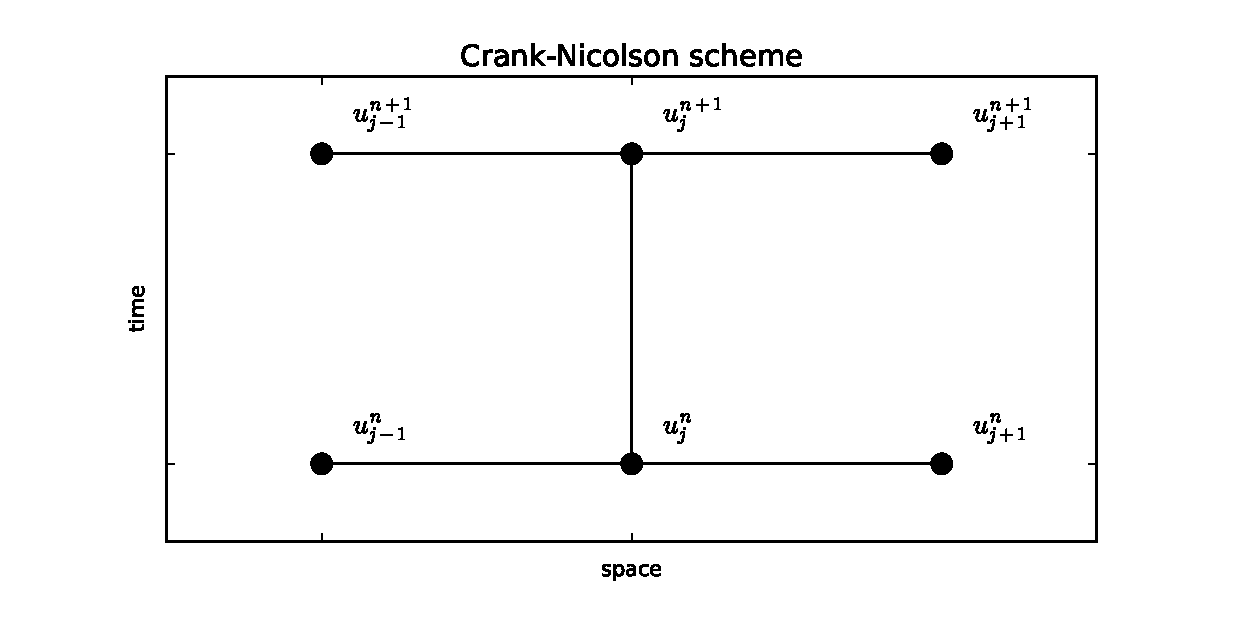
\includegraphics[width=\textwidth]{CNfootprint.eps}}
\caption{}
\label{fig:fig1}
\end{figure} \\
Як неважко бачити, завдяки подібній дискретизації нашого р-ня ми отримуємо на кожному кроці по часу систему р-нь відносно невідомих значень шуканої ф-ї у точках з індексом $(n+1)$, крім того, поки що нелінійних (через квадратичний член). Однак в подальшому ми позбавимось від цієї незручності і використаємо усі переваги даної схеми саме для лінеаризованого випадку. Розмірність такої системи $[(M+1)\times(N+1)]^2$, де $M$ та $N$ --- к-ть вузлів по осям $Ox$ і $Oy$ відповідно, як у прикладі з попереднього пункту. Отже при достатньо маленьких кроках дискретизації розв’язування подібної системи може вимагати багато обчислювальних ресурсів;
тим не менше, у лінійному випадку така система є дуже розрідженою і  має разом з граничними умовами (які в даному випадку представлені у формі Дирихле) чітко виражений 5-діагональний вид, що дозволяє нам використовувати оптимізовані формати збереження і методи розв’язання розріджених систем.

\subsection{Лінеаризація отриманої системи}
Як уже було вказано, якщо використовувати для дисткретизації \eqref{eq:fisher} схему типу Кранка-Ніколсона у її стандартному вигляді, то отримана система р-нь \eqref{eq:syst} є нелінійною, що призводить до суттєвих незручностей з обчислювальної точки зору (необхідності використовувати своєрідні, більш складні ніж для розріджених матриць, формати збереження, виключно ітераційні алгоритми розв’язку, накшталт Ньютона-Рафсона, або метод Крилова оптимізації вектор-функцій багатьох змінних, які вимагають обчислень якобіанів порядку (для нашого випадку) $[(M+1)\times(N+1)]^4$, що вимагає ресурсів ще більше, ніж зберігання 5-діагональної розрідженої матриці у звичайному ``densed'' вигляді). Тому нами запропоновано дещо інший підхід, який базується на зведенні вже отриманої системи до лінійного вигляду.

Нелінійність у \eqref{eq:syst} вносить квадратичний член $\left(\upl{0}{0}\right)^2$, отже зводити до лінійного вигляду будемо саме його. Розглянемо похідну за часом від функції $u^2(t,x,y)$:
\begin{equation}
\frac{\partial\left(u^2\right)}{\partial t} = 2u\frac{\partial u}{\partial t}
\end{equation}
що, використовуючи апроксимацію різницевим оператором по часу, може бути переписано як
\begin{equation}
\frac{\left(u^2\right)^{n+1}_{jk} - \left(u^2\right)^{n}_{jk}}{\Delta t} = \frac{2u^n_{jk}\left(u^{n+1}_{jk} - u^n_{jk}\right)}{\Delta t}
\end{equation}
звідки маємо
\begin{equation}
\left(u^{n+1}_{jk}\right)^2 = \left(u^{n}_{jk}\right)^2 + 2u^n_{jk}\left(u^{n+1}_{jk} - u^n_{jk}\right)
\end{equation}
де величини у правій частині на кожному кроці по часу відомі.
Тепер вводячи позначення $\omega_{jk} = \left(\upl{0}{0} - \un{0}{0}\right)$ і записуючи граничні (за постановкою задачі значення на границі --- константніпо часу) умови
\begin{equation}
\omega_{0,k} = \omega_{M,k} = \omega_{j,0} = \omega_{j,N} = 0
\end{equation}
ми приходимо до лінеаризованого варіанту системи \eqref{eq:syst}, яка тепер є 5-діагональною СЛАУ. Розв’язуючи її на кожному кроці відносно $\omega_{jk}$ і покладаючи $\upl{0}{0} = \omega_{jk} + \un{0}{0}$ приходимо до розв’язку початкової задачі.

\newpage
\section{Аналіз стійкості обраної різницевої схеми}
%\subsection{Попередні зауваження}
Для аналізу стійкості відповідної лінеаризованої різницевої схеми \eqref{eq:syst} будемо користуватися спектральним методом фон Неймана, детальний розгляд якого та
доведення відповідних теорем необхідності та достатності (в першу чергу для лінійного випадку) можна знайти у \cite{godun, richt}. 

Для початку визначимо згідно з \cite{godun} різницеву схему як \textit{стійку відносно збурень вхідних даних}, якщо для її розв’язку виконано:
\begin{equation}
\smash{\displaystyle\max_{j,k} |\un{0}{0}|} \le  C\smash{\displaystyle\max_{j,k} |u^0_{j,k}|},\  \forall n = 0, \dots, T,\ C = const,\ |C| < \infty
\end{equation}
для довільної обмеженої ф-ї $u^0_{j,k} = \psi_{j,k}$.

Слідуючи за \cite{richt} знайдемо коефіцієнт переходу (підсилення) $\xi$ для Фур’є-компоненти точного розв’язку різницевої схеми. Для нелінійних ДРЧП де-факто він залежить не лише від набору констант, що характеризують р-ня, і обраних кроків сітки, але й, власне кажучи, від самих розв’язків, що отримуються, тому можна лише сподіватись, що стійкість буде мати місце до деякого моменту часу $t_1$; крім того часто строгі аналітичні оцінки на коефіцієнт переходу є важкими і громіздкими, тому у даній роботі перевірку отриманої умови (в якій є явна залежність від $u^n_{j,k}$) було реалізовано у програмному коді і у випадку коли умова перестає виконуватись моделювання припинялось (в якості покращення методу, можна було б підганяти крок по часу, щоб задовільнити умову стійкості).

Розглянемо n-ту Фур’є-компоненту точного розв’язку схеми: $\un{0}{0} = \xi^ne^{imj\Delta x}e^{ilk\Delta y}$; підставимо її у \eqref{eq:syst} з лінеаризованим квадратичним членом і після скорочень, виражаючи $\xi$ отримаємо:
\begin{equation}
\xi = \frac{1 - (1-\lambda)\left[\Delta t\alpha m_0 + 2\psi\left(m\Delta x, l\Delta y\right)\right] - (1-2\lambda)\Delta t\alpha\beta\times u^n\left(m\Delta x, l\Delta y\right)}
{1 - \lambda\left[\Delta t m_0\alpha - 2\psi\left(m\Delta x, l\Delta y\right)\right] + 2\lambda\Delta t\alpha\beta\times u^n\left(m\Delta x, l\Delta y\right)} \label{eq:stable}
\end{equation}
де $\psi(m\Delta x, l\Delta y) = S_x\{1-\cos(m\Delta x)\} + S_y\{1-\cos(l\Delta y)\}$, $S_x = \frac{\sigma\Delta t}{\Delta x^2},\ S_y = \frac{\sigma\Delta t}{\Delta y^2}$ --- відповідні числа дифузії.

Відомо, що необхідною умовою стійкості є
\begin{equation}
\smash{\displaystyle\max_{m,l} |\xi|} < 1
\end{equation}
отже саме її і будемо використовувати у програмній реалізації.
\newpage
\section{Опис програмної реалізації}
\subsection{Об’єктна модель}
Програмна реалізація розв’язку р-ня \eqref{eq:fisher} була розроблена за допомогою мови Python, версія 2.7.6, та додаткових програмних пакетів для деяких специфічних задач лінійної алгебри, що виникають у процесі розв’язку, а саме: \textbf{scipy (0.17.0)} (для представлення розрідженої матриці системи у форматі DIAGONAL та використання відповідних солверів для розріджених систем) та \textbf{numpy (1.11.0)} для базових представлень масивів та операцій лінійної алгебри. Відповідні лістинги наведені у \textbf{Додатку І}.

Об’єктна модель реалізації складається з двох класів: \textbf{CNModel} та \textbf{CNSolver}.
Перший репрезентує модель задачі, тобто зберігає в якості своїх атрибутів параметри рівняння та схеми дискретизації, функцію, що задає початкові та граничні умови, а також інкапсулює реалізацію методів, що готують модель для розв’язання та є основними методами, які викликає клієнтський код солвера.
Нижче наведено параметри, що передаються в конструктор класу при створенні моделі:
\vspace{10pt}
\begin{center}
	\begin{tabular}{|l|c|}
	\hline
	Parameters & Description \\ \hline
	alpha, beta, m\_0, sigma & $\alpha, \beta, m_0, \sigma$ --- Параметри р-ня (\textbf{float}) \\ \hline
	dt, dx, dy & $\Delta t, \Delta x, \Delta y$ --- кроки по часу, $Ox$, $Oy$ відповідно (\textbf{float})  \\ \hline
	T, M, N & Кількість вузлів по часу, $Ox$, $Oy$ відповідно (\textbf{integer}) \\ \hline
	lambd & $\lambda$ --- ваговий коеф-т (\textbf{float, belongs to [0, 1]}) \\ \hline
	init\_cond & $U(\vec{x})$ --- ф-я початкових умов (\textbf{either callable or float}) \\ \hline
	\end{tabular}
\end{center}
\vspace{10pt}
Методи классу включають в себе (Listing 1, Додаток І): \textbf{\_get\_footprint}, що одноразово обчислює коеф-ти в системі рівнянь, які стоять в кожному рядку при відповідних членах, \textbf{get\_initial\_state}, що формує сітку початкових значень, \textbf{prepare}, що є основним методом, який викликає клас \textbf{Solver}, і який готує модель до запуску солвера, ініціалізуючи всі необхідні параметри та \textbf{stability\_factor}, що обчислює значення у вузлі $(i\Delta x, j\Delta y)$ ф-ї $\psi$, яка виникає у виразі для коеф-та підсилення \eqref{eq:stable}.

Другий клас є своєрідним фреймворком для проведення усіх операцій (основних та підготовчих) по розв’язуванню задачі та відповідному зберіганню розв’язків; він жорстко зв’язується з моделлю, яку ми передаємо йому (\textbf{CNSolver.fit(CNModel)}). Для розв’язання кожної зі згенерованих моделей повинен бути створений свій солвер, у який "фітиться" модель і який агрегує відповідні розв’язки. Розв’язки у буфері солвера у процесі обробки зберігаються у так званій \textit{flat} моделі --- сітка, представлена у вигляді одновимірного numpy-масиву, рядок за рядком. Після обробки матричний вигляд відновлюється і записується у остаточний багатовимірний numpy-масив, кожен елемент якого представляє розв’язок на деякому кроці часу.

У наступному пункті ми розглянемо специфічні методи роботи з розрідженими масивами даних, які використовуються класом \textbf{CNSolver} для динамічної генерації  матриці системи у відповідному представленні та для оптимального розв’язання системи, представленої у подібному вигляді.\\

\subsection{Формати представлень розріджених масивів. Проекційні алгоритми}
Генерувати матрицю системи необхідно на кожній ітерації, оскільки її коеф-ти явно залежать від $\un{0}{0}$, саме тому цю допоміжну операцію було реалізовано всередині класу \textbf{CNSolver} --- відповідні значення додатково зберігаються у флет-моделі у буфері солвера і допомагають генерації. Як бачимо це вимагає значних витрат обчислювальних ресурсів, в тому числі й пам’яті машини, особливо якщо вимагати достатньо високої точності розв’язку. Матриця системи, як було вже вказано, є 5-діагональною і, за рахунок цього, дуже сильно розрідженою. Тому нами був використаний динамічний метод заповнення матриці виключно ненульовими ел-ми і подальше її конвертування в формат \textbf{DIAGONAL}. Сам формат описаний нижче. Динамічне заповнення забезпечив модуль \textbf{scipy.sparse}, у якому реалізований допоміжний формат \textbf{lil\_matrix}, який є своєрідним узагальненим шаблоном для будь-якого формату збереження розріджених матриць. Він дозволяє додавати ненульовий елмент з вказанням конкретної позиції і в подальшому трансформувати матрицю для використання у солвері.

У нашій реалізації ми використовували формат представлення \textbf{DIAGONAL}, на противагу іншому найбільш розповсюдженому формату \textbf{CSR} (Compressed Sparse Row), оскільки він безпосередньо був розроблений для n-діагональних розріджених матриць і конвертація у нього для таких матриць виконується дещо швидше. Детальний огляд конкретних форматів збереження можна знайти у \cite{saad}.

Збереження у форматі \textbf{DIAGONAL} передбачає наступне. Діагоналі зберігаються у прямокутному масиві \textbf{DIAG} розмірності $n\times Nd$, де Nd --- к-ть ненульових діагоналей. Кожень стовпець представляє діагональ і у діагоналей, що мають менше n елементів на відповідних позиціях стоять деякі фіктивні "заповнювачі". Зсуви діагоналей відносно головної мають бути відомі і записуються вони у окремий одновимірний масив \textbf{IOFF} довжини Nd. Значення 0 відповідає головній діагоналі, -1 --- першій субдіагоналі у нижньому трикутнику, +1 --- першій супердіагоналі у верхньому трикутнику і т.д. Послідовність вектор-стовпчиків, що представляють діагоналі та їх зсувів у масиві \textbf{IOFF} повинні співпадати, при цьому абсолютне розташування самих вектор-стовпчиків відносно один одного у \textbf{DIAG} зазвичай суттєвого значення не має, хоча в деяких випадках може бути корисним прямий порядок.

Система р-нь, що представлена розрідженою матрицею $LHS$ та вектор-стовпчиком $RHS$, що генеруються солвером на кожному кроці, представлена у специфічному форматі і повинна розв’язуватись за допомогою відповідних алгоритмів. Модуль \textbf{scipy.sparse.linalg} пропонує для розріджених матриць серію різних алгоритмів, що мають свої переваги та недоліки і ефективність та застосовність яких часто сильно залежить від властивостей матриці лівої частини системи, тому перед нами постала проблема вибору найкращого із доступних методів. Нами було проведено невелике дослідження швидкості обробки кожним з алгоритмів системи великих розмірностей ($90601\times90601 \approx 13$Mb у серіалізованому вигляді). Для кожного алгоритму проводилась серія запусків для 5 матриць однакової розмірності, вказаної вище, згенерованих солвером на першому кроці по часу для моделей з різним набором параметрів і записаних у дамп-файл. Абсолютна точність наближення задавалась порядку $10^{-6}$, на противагу значенню за замовчуванням для даного модуля: $10^{-4}$; початкове наближення явно не задавалось, так що за замовчуванням алгоритм стартував зі значення $\vec{0}$. Час виконання був усереднений для кожного з алгоритмів і наведений у таблиці нижче.
\vspace{10pt}
\begin{center}
	\begin{tabular}{|l|c|}
	\hline
	Algorithm & Time of estimation, sec \\ \hline
	GMRES & $1.77282$ \\ \hline
	QMR & $1.83367$ \\ \hline
	BiCGSTAB & $0.97049$\\ \hline
	LGMRES & $1.72245$\\ \hline
	\end{tabular}
\end{center}
\vspace{10pt}
Неважко, бачити, что суттево швидшим ніж інші є BiCGSTAB (Biconjugate Gradient Stabilised Algorithm), отже в якості солвера для нашої системи був обраний саме він.

Зробимо невелике зауваження щодо класу пропонованих алгоритмів. Всі вони детально розглянуті у \cite{saad}. Клас даних алгоритмів називається \textit{проекційними алгоритмами на підпростір Крилова}, або просто \textit{алгоритмами криловського типу}. Усі проекційні алгоритми спираються на ключову ідею, що чергове наближення для розв’язку лінійної системи $\bf A x = \bf b$ може бути шукане в деякому підпросторі $\mathbb{K}_m$ розмірності $m$ основного простору $\mathbb{R}^n$, який називається \textit{subspace of candidate approximants} і для забезпечення цього має бути накладено $m$ умов, що де-факто є умовами ортогональності шуканого наближення (якщо говорити більш точно, то чергової нев’язки, а не власне самого наближення) до $m$ базисних векторів іншого підпростору $\mathbb{L}_m$, який називають \textit{subspace of constraints}. Усі алгоритми криловського типу мають важливу спільну особливість: в якості $\mathbb{K}_m$ на кожному кроці $m$ обирається підпростір Крилова $\mathbb{K}_m(\textbf{A},\vec{v}) = span(\vec{v}, \textbf{А}\vec{v}, \dots, \textbf{А}^{m-1}\vec{v})$ для деякого вектора $\vec{v}$, який найчастіше покладають рівним $\vec{r}_0$ --- початковій нев’язці; тут \textbf{А} --- матриця системи, що розв’язується. Уся різноманітність алгоритмів криловського типу полягає у різних методах генерації базису чергової лінійної оболонки та відповідних апріорних припущеннях щодо вигляду матриці $\textbf{А}$. Чудовий опис алгоритму побудови біортогональних систем базисів для двох криловських підпросторів, один з яких спирається на саму матрицю $\textbf{А}$, а інший на $\textbf{А}^T$, і який є ключовим для обраного нами алгоритму  BiCGSTAB, можна знайти у оригінальній роботі автора даного алгоритму \cite{lanczos}.
\newpage
\section{Аналіз отриманих результатів}
Запуски програмної реалізації проводились здебільшого на сітках $101\times 101$ та $201\times 201$ для квадратних областей $[0,1]\times [0,1]$ та $[0,10]\times [0,10]$ з однаковими просторовими кроками $0,01$ та $0,1$ відповідно. Моделювання проводилось для 50 кроків по часу. Для $\lambda = 0,5, \lambda = 0,75$ обирався крок по часу $\Delta t = 0,01$, для $\lambda = 0,25$ (0 --- явна схема) заради забезпечення стійкості крок по часу обирався меншим, а саме у випадку $\Delta x = \Delta y = 0,01$ покладали $\Delta t = 0,0001$ і проводили моделювання для 100 кроків по часу. В якості $U(\vec{x})$ --- функції початкових умов була обрана гаусіана
\begin{equation}
2\left[exp\left\{-\frac{(x-0,5)^2}{2}\right\} + exp\left\{-\frac{(y-0,5)^2}{2}\right\}\right]
\end{equation}
для квадрату $[0,1]^2$ та
\begin{equation}
3\left[exp\left\{-\frac{(x-3)^2}{2\times 1,5^2}\right\} + exp\left\{-\frac{(y-2,5)^2}{2\times 1,5^2}\right\}\right]
\end{equation}
для квадрату $[0,10]^2$.
Графіки для цих двох випадків, представлені у формі heat-plot, наведено у \textbf{Додатку ІІ}.

Крім того, було проаналізовано порівняльну поведінку точності розв’язків при однакових кроках дискретизації абсолютно явної схеми без додаткової лінеаризації, що її описано у підрозділі 2.3, та пропонованої неявної схеми при $\lambda = 0.5\ (0,75)$. З апріорних оцінок відомо, що неявна схема має по часу вищий порядок точності, ніж явна, проте виникло питання, наскільки швидко у явній схемі накопичуються похибки. Проводилось моделювання при $\Delta t = 0,001\ \Delta x = \Delta y = 0,1\ $ на $[0,10]^2$ для 5 кроків по часу. Порівняння проводилось шляхом оцінки норми Фробеніуса різниці матриць, що представляють розв’язок, для кожного кроку по часу. Задавалась точність, з якою ці матриці повинні співпадати. У таблиці нижче наведено результати порівнянь. 
\begin{center}
	\begin{tabular}{|l|l|}
	\hline
	$\epsilon = 0.001$ & Is equal? \\ \hline
	1 & True \\ \hline
	2 & True \\ \hline
	3 & False \\ \hline
	4 & False \\ \hline
	5 & False \\ \hline
	\end{tabular}
\end{center} 
\vspace{10pt}
Як бачимо, вже після другого кроку по часу результати починають відрізнятись більше ніж на $0,001 = \Delta t$, тобто накопичення похибок у явній схемі відбувається катастрофічно швидко.

Ще одним суттєвим результатом є той факт, що в нелінійних моделях умова стійкості фон Неймана є лише необхідною, але не достатньою, внаслідок залежності коеф-ту підсилення від отриманого на поточному кроці результату розв’язання. На графіках нижче наведено результат моделювання для 5 кроків по часу на $[0,10]^2$ при тій же початковій ф-ї, що вказана вище і при таких значеннях параметрів моделі: $\alpha = -10,\ \beta = -1,\ m_0 = 2,\ \sigma = -0,01,\ \lambda = 0,75, \Delta t = 0,01, \Delta x = \Delta y = 0,1$. При цій комбінації параметрів умова фон Неймана для \eqref{eq:stable} виконується для всіх 5-ти кроків, при цьому на границі, де ф-я початкових умов, як і функція розв’язку швидко змінює характер росту і стрімко спадає, ми можемо бачити прояви нестійкості коливного харакеру.
\vspace{10pt}
\addtwoimghere{nonst2}{nonst3}{1}
\vspace{10pt}
\addtwoimghere{nonst4}{nonst5}{1}
\newpage
%\input{finally}
\newpage
\anonsection{Додаток I}

\lstinputlisting[label=CNModel,caption=class CNModel]{../Linearized_CN/CNModel-clear.py}
\newpage
\lstinputlisting[label=CNSolver,caption=class CNSolver]{../Linearized_CN/CNSolver-clear.py} % Should be reconstruct into appendix
\newpage
\anonsection{Додаток II}
Нижче наведено графіки для $\lambda = 0,75,\ \Delta t =0,01,\ \Delta x=\Delta y=0,01,\ \alpha =1,\ \beta=1,\ \sigma=1$
\vspace{20pt}
\addtwoapp{0}{001}{1.35}
\addtwoapp{003}{005}{1.35}
\newpage
\vspace{25pt}
\addtwoapp{007}{011}{1.35}
\addtwoapp{047}{048}{1.35}
\newpage
\vspace{25pt}

Нижче наведено графіки для $\lambda = 0,5,\ \Delta t =0,01,\ \Delta x=\Delta y=0,1,\ \alpha =1,\ \beta=1,\ \sigma=1$
\vspace{20pt}
\addtwoapp{t0}{t002}{1.35}
\addtwoapp{t005}{t011}{1.35}
\newpage
\vspace{25pt}
\addtwoapp{t015}{t028}{1.35}
\addtwoapp{t039}{t047}{1.35}
\newpage
\renewcommand{\refname}{Список використаних джерел}
\begin{thebibliography}{8}
\bibitem{godun}Годунов С.К., Рябенький В.С. Разностные схемы. Введение в теорию. Изд.2, перераб. и доп. — Наука, 1977, 440 с.
\bibitem{richt}\href{https://issuu.com/fwebsite/docs/rixtmajer_morton_raznostnie_metody_}{Рихтмайер Р., Мортон К. Разностные методы решения краевых задач: Пер. с англ. — М.:Мир, 1972, 420 с.}
\bibitem{fisher}\href{https://digital.library.adelaide.edu.au/dspace/bitstream/2440/15125/1/152.pdf}{R. A. Fisher. The wave of advance of advantageous genes, Ann. Eugenics 7:353–369, 1937}
\bibitem{lanczos}\href{https://archive.org/details/jresv49n1p33}{C. Lanczos, Solution of linear equations by minimized iterations, J. Res. Natl. Bur. Stand., 49 (1952), pp. 33–53.}
\bibitem{bio}\href{https://books.google.com.ua/books?id=0pOKCgAAQBAJ&printsec=frontcover&hl=uk#v=onepage&q&f=false}{B. Perthame, Parabolic Equations in Biology: Growth, reaction, movement and diffusion, Springer, 2015}
\bibitem{saad}\href{http://www-users.cs.umn.edu/~saad/IterMethBook_2ndEd.pdf}{Y. Saad, Iterative Methods for Linear Systems, SIAM, 2003.}
\bibitem{treft}\href{http://people.maths.ox.ac.uk/trefethen/pdectb/fisher2.pdf}{L. N. Trefethen, K. Embree, The PDE Coffee Table Book, Unpublished, 2001}
\end{thebibliography}
\end{document}
